\documentclass{article}
\usepackage{amsmath,amsthm,amssymb}
\usepackage {mathtext}
\usepackage{amsfonts} 
\usepackage[T1,T2A]{fontenc}
\usepackage[utf8]{inputenc}
\usepackage [english, russian] {babel}
\usepackage[babel=true]{microtype}
\usepackage{caption}
\usepackage{subcaption}
\captionsetup[table]{position=t,justification=raggedleft,slc=off}
\setlength{\abovecaptionskip}{0pt}
\usepackage {geometry}
\usepackage{graphicx}
\geometry{margin=1in}
\title{Лабораторная работа №1.4.5 \\ Изучение колебаний струны}
\author{Павел Рудачихин \\ Б04-507}
\date{13.11.2025}
\begin {document}
\maketitle{}
\section* {Аннотация} 

\hspace{4mm} \textbf{Цель работы:} изучить поперечные стоячие волн на тонкой натянутой струне;
измерить собственные частоты колебаний струны и проверить условие образования стоячих волн; 
измерить скорость распространения поперечных волн на струне и исследовать её зависимость от натяжения струны.

\textbf{В работе используются:} закрепленная на станине стальная струна, набор грузов, электромагнитные датчики, звуковой генератор, двухканальный осциллограф, частотомер.

\textbf{Методы:} 1) определение  углового  коэффициента  наклона  зависимости двух величин; 2) измерение массы тел с помощью весов.

\section* {Теоретические сведения}
\subsection* {Струна}

\hspace{4mm} \textbf{Струной} в акустике называют однородную тонкую гибкую упругую нить. В данной работе изучаются поперечные колебания стальной струны, натянутой горизонтально и закрепленной между двумя неподвижными зажимами.
Основное свойство струны — \textbf{гибкость} — обусловлено тем, что её по перечные размеры малы по сравнению с длиной. Это означает, что напряжение в струне может быть направлено только вдоль неё.
В натянутой струне возникает \textbf{поперечная упругость}, т.е. способность сопротивляться всякому изменению формы, происходящему без изменения объема. При вертикальном смещении произвольного элемента струны возникают силы, действующие на соседние элементы, и вся струна приходит в движение в вертикальной плоскости. Передача возбуждения представляет собой поперечные бегущие волны, распространяющиеся с некоторой скоростью в обе стороны от места возбуждения.

\subsection* {Волновое уравнение}

\hspace{4mm} Направим ось $x$ вдоль струны. Форму струны
будем описывать функцией $y(x, t)$ определяющей её вертикальное смещение в точке $x$ в момент времени $t$ (см. рис. 1). Угол наклона касательной к
струне в точке $x$ относительно горизонтального направления обозначим $\alpha$. Причём $ \tg \alpha = \frac{\partial{y}}{\partial{x}} $

\begin{figure}[h!]
	\centering
	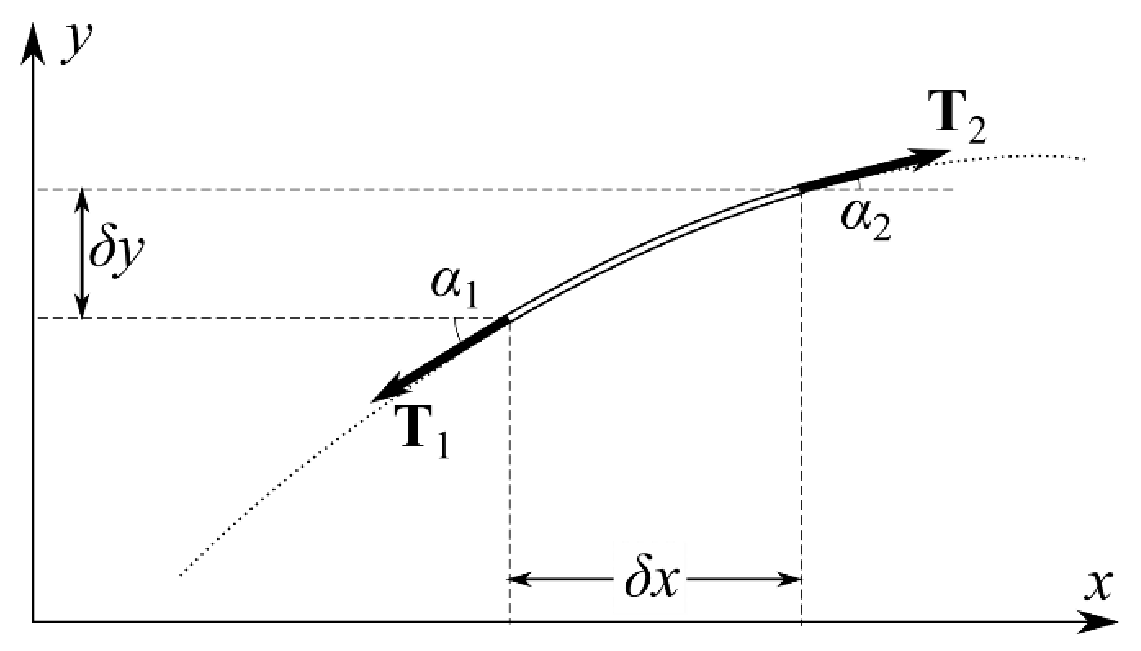
\includegraphics[width=0.5\linewidth]{1}
	\caption{К выводу уравнения колебаний струны: $\delta x, \delta y$ - проекции участка струны, $T_1, T_2$ - силы натяжения на концах участка, $\alpha_1, \alpha_2 $ - углы наклона касательных к струне на концах участка.}
	\label{fig:1}
\end{figure}

Рассмотрим элементарный участок струны, находящийся в точке $x$ ,
имеющий длину $\delta x$ и массу $\delta m = \rho \delta x$, где $\rho$ — \textit{погонная плотность} струны (масса на единицу длины). При отклонении от равновесия
на выделенный элемент действуют силы натяжения $T_1$ и $T_2$, направленные
по касательной к струне. Заметим, что угол
$\alpha$ зависит от координаты $x$ вдоль струны и различен в точках приложения
сил $T_1$ и $T_2$. Таким образом, второй закон Ньютона для вертикального движения элемента струны имеет вид:

\begin{equation}
	\delta m \frac{\partial{}^2 y}{\partial{x^2}} = -T_1 \sin \alpha_1 + T_2 \sin \alpha_2
\end{equation}

Так как колебания струны малы, можно сделать несколько упрощений: $T_1 \approx T_2 =: T$ и $\alpha \approx \sin \alpha \approx \tg \alpha = \frac{\partial{y}}{\partial{x}}$

Разделим обе части уравнения на $\delta x \rightarrow 0$. Введём величину $u = \sqrt{\frac{T}{\rho}} $ с размерностью скорости. Имеем \textit{волновое уравнение}:

\begin{equation}
	\frac{\partial{}^2 y}{\partial{t^2}} = u^2 \frac{\partial{}^2 y}{\partial{x^2}}
\end{equation}

\subsection* {Бегущие волны}

\hspace{4mm} Заметим, что произвольная функция вида $y = f(x - ut)$ является решением уравнения (2). Такая функция описывает возмущение струны произвольной формы, которое смещается поступательно со скоростью $u$ вдоль оси $x$, не меняя своей формы. 

Известно, что общее решение дифференциального уравнения в частных производных (2) представимо в виде
суммы двух волн произвольной формы, бегущих в противоположные стороны с одинаковыми скоростями:	$y(x,t) = y_1(x - ut) + y_2(x + ut)$. Особый интерес представляет случай гармонических колебаний:

\begin{equation}
	y(x, t) = a \cos (k(x + ut)) + b \cos (k(x - ut)) = a \cos (\omega t + kx) + b \cos (\omega t - kx),
\end{equation}

где $ k = \frac{2\pi}{\lambda}$ - волновое число ($\lambda$ - длина волны), $u = \frac{\omega}{k}$ - скорость бегущей волны. Введём $\nu = \frac{\omega}{2\pi}$ - частота волны.

\subsection* {Стоячие волны}

\hspace{4mm} Так как концы струны закреплены, $y(0, t) = y(L, t) = 0$, где $L$ - длина закреплённого участка струны. Подставив эти условия в уравнение (3), получим уравнение стоячей волны:

\begin{equation}
	y(x, t) =  2a \sin kx \cdot \sin \omega t,
\end{equation}

причём на длине струны укладывается целое число полуволн (см. рис. 2):

\begin{equation}
	n \cdot \frac{\lambda_n}{2} = L, \ \ \ n \in \mathbb{N},
\end{equation}

поэтому струна может колебаться только с определёнными \textit{собственными частотами}:

\begin{equation}
	\nu_n = \frac{n}{2L}\sqrt{\dfrac{T}{\rho}}, \ \ \ n \in \mathbb{N}
\end{equation}

\begin{figure}[h!]
	\centering
	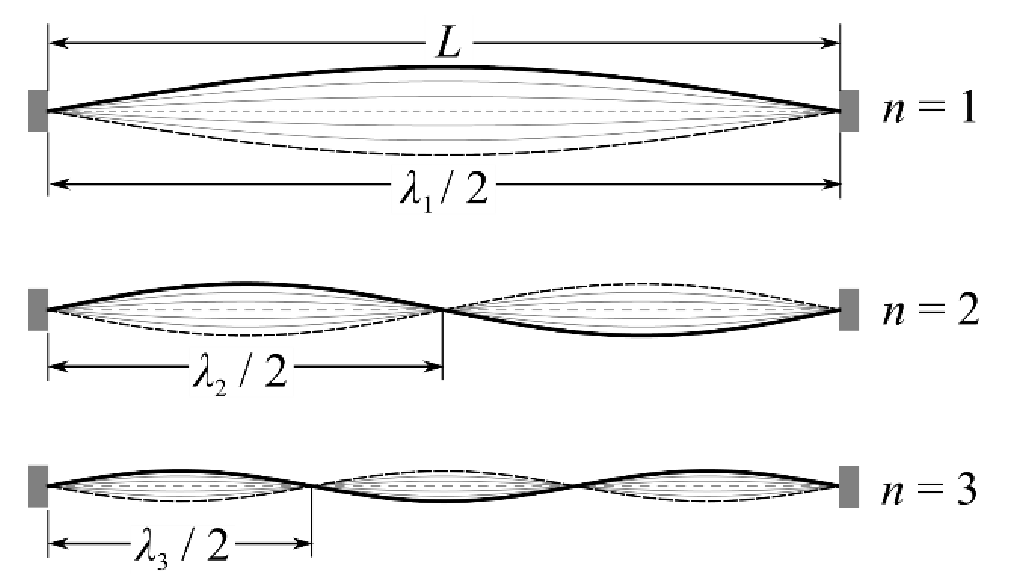
\includegraphics[width=0.5\linewidth]{2}
	\caption{Стоячие волны собственных частот с $n = 1, 2, 3$}
	\label{fig:2}
\end{figure}


\subsection* {Резонанс}


\hspace{4mm} Для поддержания незатухающих стабильных колебаний используется явление резонанса: вынуждающая частота совпадает с собственной частотой струны, благодаря чему можно наблюдать стоячие волны. Для этого достаточно одного точечного источника колебаний: несмотря на то, что стоячая волна не переносит энергию, из-за потери при отражении от креплений возникает бегущая волна (малая по сравнению со стоячей), которая и выступает переносчиком энергии.

\section*{Экспериментальная установка}

\begin{figure}[h!]
	\centering
	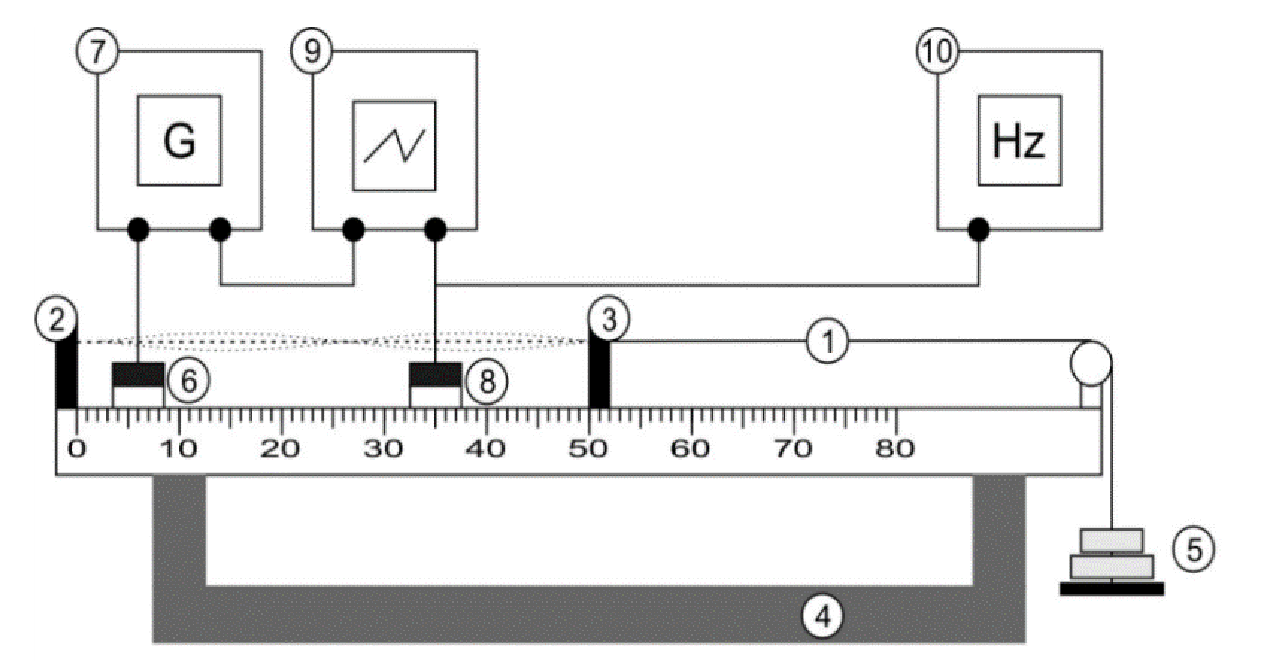
\includegraphics[width=0.7\linewidth]{3}
	\caption{Экспериментальная установка: 1 - струна, 2,3 - стойки, 4 - станина, 5 - платформа с грузами, 6 - возбуждающий датчик, 7 -генератор, 8 - регистрирующий датчик, 9 - осциллограф, 10 - частотомер}
	\label{fig:3}
\end{figure}

 Схема установки приведена на рис. 3. Стальная струна 1 закрепляется в горизонтальном положении между двумя стойками с зажимами 2 и 3, расположенными на станине 4. Один конец струны 
закреплен в зажиме 2 неподвижно. К противоположному концу струны, перекинутому через блок, прикреплена платформа с грузами 5, создающими натяжение струны. Зажим 3 можно передвигать по станине, устанавливая требуемую длину струны. Возбуждение и регистрация колебаний струны осуществляются  с  помощью  электромагнитных  датчиков, 
расположенных на станине под струной. Электромагнитный датчик 6 подключен  к  звуковому  генератору 7  и  служит  для  возбуждения  колебаний 
струны, частота которых измеряется с помощью частотомера 10 ( частотомер встроен в генератор). Колебания струны регистрируются с помощью электромагнитного датчика 8, сигнал с которого 
передается на вход осциллографа 9. 

\subsection* {Принцип работы датчиков}

\begin{figure}[h!]
	\centering
	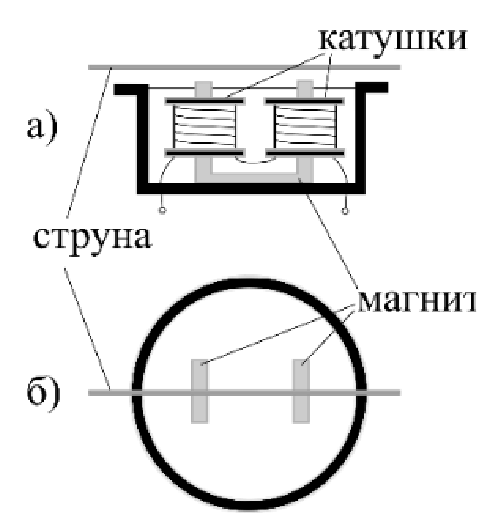
\includegraphics[width=0.2\linewidth]{4}
	\caption{Электромагнитный датчик: а) вид сбоку, б) вид сверху}
	\label{fig:4}
\end{figure}

\hspace{4mm} Устройство и внешний вид электромагнитного датчика показаны на рис. 4. Магнитное поле в зазоре между полюсами складывается из постоянного поля магнита $B_0$ и переменного поля катушек $B$, причём $B \ll B_0$. Сила, действующая на струну, пропорциональна квадрату индукции суммарного магнитного поля, но прямо пропорциональна индукции переменного магнитного поля, т.к. $B^2$ слишком мал:

\begin{equation}
	F \propto (B_0 + B)^2 \approx B_0^2 + 2B_0B
\end{equation}

$B$, в свою очередь, прямо пропорциональна току в катушке $I$. Поэтому $F \propto I$, и частота вынуждающих колебаний совпадает с частотой звукового генератора.



\section*{Используемое оборудование}

\hspace{4mm} В данной работе для измерения массы использованы цифровые \textbf{весы}. Погрешность измерения массы определена как три в последнем разряде дисплея прибора: $\Delta_{\text{m}} = \pm 0,3$ г

Погрешность \textbf{линейки} составляет $\Delta_{\text{Л}} = \pm 0,5$ мм 

В работе использованы двухканальный \textbf{осциллограф} GOS-620 с полосой пропускания 20 МГц и \textbf{генератор-частотомер} АКИП-3408/3.

\section*{Результаты измерений и наблюдений}

\hspace{4mm} Параметры экспериментальной установки приведены в таблице 1.  

\begin{table}[h!]
	\centering
	\captionbox{Параметры установки}{
		\begin{tabular}{|c|c|}
			\hline
			Параметр  & Значение  \\
			\hline
			Диаметр струны, $d$ & $(0,30 \pm 0,01)$ мм \\
			\hline
			Погонная плотность, $\rho$  & 568,4 мг/м  \\
			\hline
			Длина струны, $L$  & $(500 \pm 1)$ мм \\
			\hline
			Масса подвеса, $m_0$  & $(119,5 \pm 0,1)$ г \\
			\hline
	\end{tabular}}
\end{table}

Полученные значения резонансных частот 1-10 гармоник для 4 разных грузов представлены в таблице 2.

\begin{table}[h!]
	\centering
	\captionbox{Резонансная частота}{
	\begin{tabular}{|r|r|r|r|r|r|r|r|r|r|r|}
		\hline
		Масса груза, г& $\nu_1$, Гц    & $\nu_2$, Гц      & $\nu_3$, Гц     & $\nu_4$, Гц       & $\nu_5$, Гц      & $\nu_6$, Гц   & $\nu_7$, Гц  & $\nu_8$, Гц  & $\nu_9$, Гц  & $\nu_{10}$, Гц \\
		\hline
		1073,5   & 136      & 274      & 409      & 550      & 685      & 828      & 964      & 1092     & 1246     & 1360 \\
		\hline
		1524,2   & 161      & 322      & 483      & 645      & 806      & 969      & 1132     & 1290     & 1463     & 1628 \\
		\hline
		2023,3   & 187      & 373      & 561      & 748      & 936      & 1125     & 1314     & 1503     & 1694     & 1885 \\
		\hline
		2505,0   & 208      & 416      & 624      & 832      & 1041     & 1249     & 1460     & 1670     & 1881     & 2092 \\
		\hline
	\end{tabular}}
\end{table}

Для определения амплитудно-частотной характеристики струны получена зависимость амплитуды напряжения от частоты вынуждающих колебаний, представленная в таблице 3.

\begin{table}[h!]
	\centering
	\captionbox{Зависимость амплитуды напряжения от частоты вынуждающих колебаний}{
	\begin{tabular}{|r|r|r|r|r|r|r|r|r|r|r|r|r|}
		\hline
		$\nu$, Гц& 206,8    & 206,9    & 207,0    & 207,1    & 207,2    & 207,3    & 207,4    & 207,5    & 207,6    & 207,7    & 207,8    & 207,9 \\
		\hline
		$U$, 5 мВ & 1,0      & 1,5      & 2,0      & 2,5      & 3,0      & 3,0      & 4,0      & 4,0      & 3,0      & 2,0      & 1,5      & 1,0 \\
		\hline
	\end{tabular}}
	\label{tab:addlabel}%
\end{table}%

При частоте вынуждающих колебаний, равной половине первой гармоники, на осциллографе в режиме X-Y наблюдалась устойчивая фигура Лиссажу с одним самопересечением - эллипс (см. рис. 5).

\begin{figure}[h!]
	\centering
	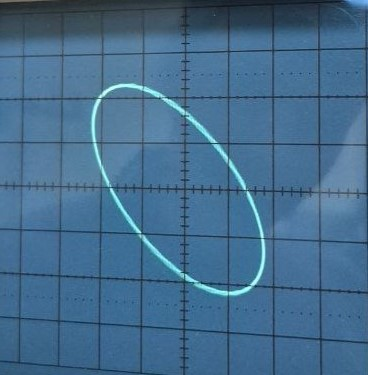
\includegraphics[width=0.5\linewidth]{8}
	\caption{Фигура Лиссажу при частоте вынуждающих колебаний на половинной гармонике}
	\label{fig:8}
\end{figure}


\section*{Обработка результатов}
\hspace{4mm} Погрешность измерения массы грузов возрастает при добавлении грузов, т.к. итоговая масса есть сумма измеренных масс. Погрешность суммы определена по формуле:

\begin{equation}
	\sigma_{m_1 + m_2} = \sqrt{\sigma_{m_1}^{2} + \sigma_{m_2}^{2}}
\end{equation}

Методика измерения резонансной частоты основана на подборе её значения на генераторе. В ходе работы подбор осуществлялся с точностью до 1 Гц. Это значение примем за систематическую погрешность измерения частоты. 

\begin{figure}[h!]
	\centering
	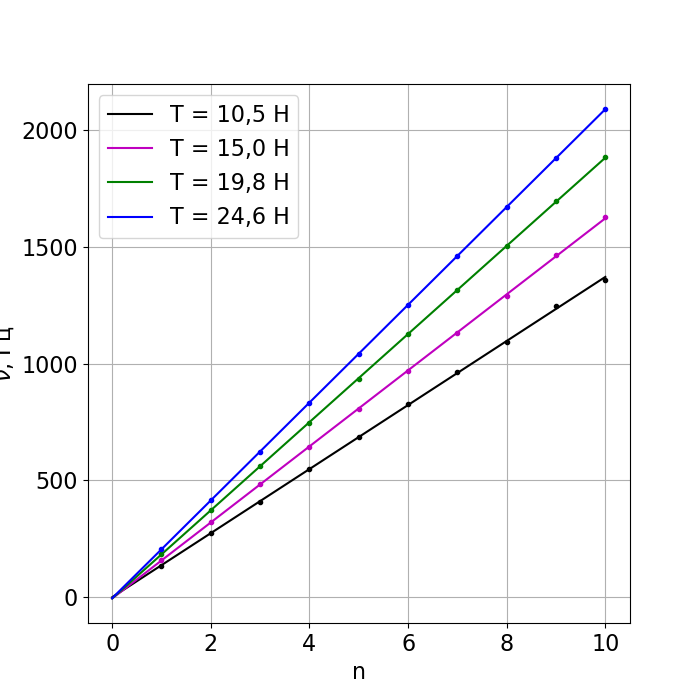
\includegraphics[width=0.7\linewidth]{5}
	\caption{График зависимости $\nu = \nu(n)$ для четырёх разных масс грузов}
	\label{fig:5}
\end{figure}

Нанесём полученные экспериментально точки на график $\nu = \nu(n)$ (частоты от номера гармоники). По методу наименьших квадратов проведём наилучшую прямую (см. рис. 6). Заметим, что все прямые с высокой точностью проходят через начало координат. Полученный угловой коэффициент $k_1$ связан со скоростью бегущей волны $u$ следующим образом (по формуле (6)):

\begin{equation}
	\nu = k_1 n = \frac{u}{2L} n; \ \ \ u = 2 L k_1
\end{equation}

C помощью метода наименьших квадратов также определена случайная погрешность углового коэффициента. Полная погрешность здесь и далее определена так:

\begin{equation}
	\sigma_{полн} = \sqrt{\sigma_{случ}^2 + \sigma_{сист}^2}
\end{equation}

Относительная погрешность измерения скорости вычислена по формуле:

\begin{equation}
	\varepsilon_u =  \sqrt{\varepsilon_L^2 + \varepsilon_{k_1}^2}
\end{equation}

Получены значения скоростей бегущей волны для четырёх опытов:

\begin{equation}
	\boxed{u_1 = (137 \pm 1) \ м/с \ \ \ u_2 = (163 \pm 1) \ м/с \ \ \ u_3 = (189 \pm 1) \ м/с \ \ \ u_4 = (209 \pm 1) \ м/с }
\end{equation}

\begin{figure}[h!]
	\centering
	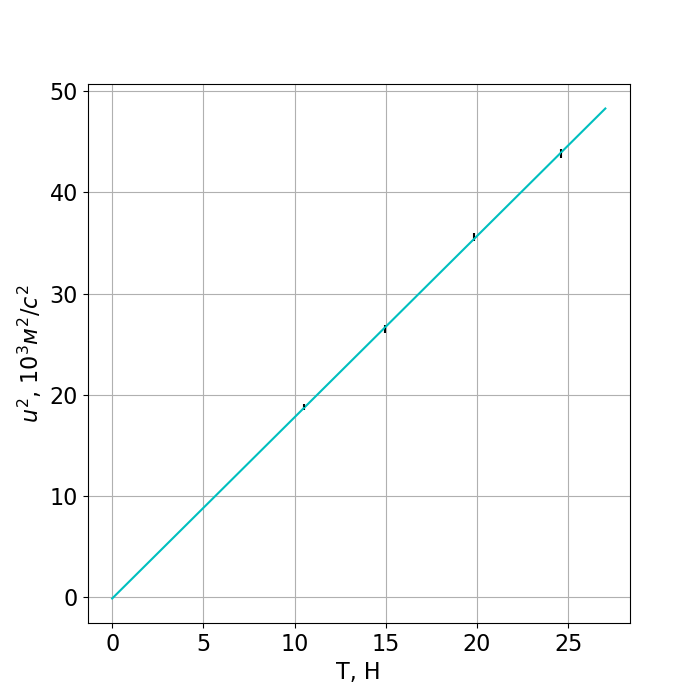
\includegraphics[width=0.7\linewidth]{6}
	\caption{График зависимости $u^2(T)$}
	\label{fig:6}
\end{figure}

Аналогично воспользовавшись методом наименьших квадратов для зависимости $u^2(T)$ (см. рис. 7), находим погонную плотность струны:

\begin{equation}
	\boxed{\rho = (559 \pm 10) \ мг/м}
\end{equation}

Все вычисления произведены с использованием программы, написанной специально для этих целей на языке программирования Python. Построение графиков выполнено с помощью модуля Matplotlib. Исходный код программы содержится в электронном приложении к работе.

\begin{figure}[h!]
	\centering
	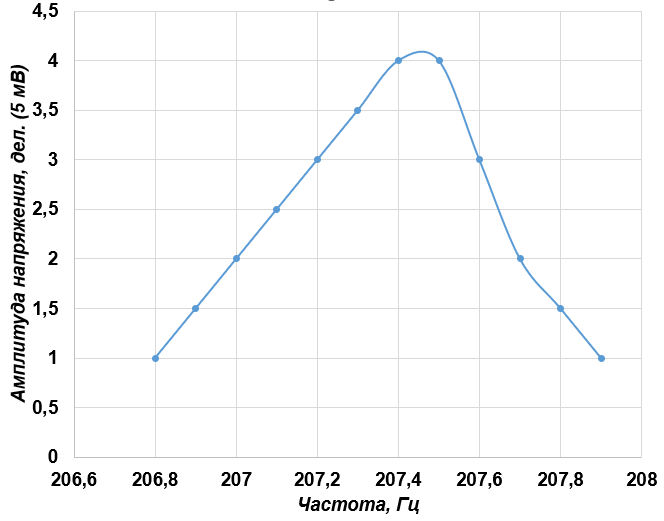
\includegraphics[width=0.7\linewidth]{7}
	\caption{Амплитудно-частотная характеристика: график зависимости $U(\nu)$}
	\label{fig:7}
\end{figure}

Амплитудно-частотная характеристика построена в ПО Microsoft Excel (см. рис. 8).

На уровне 0,7 от максимальной амплитуды напряжения (при $\nu_{рез} = 207,4$) ширина резонансной кривой составила $\Delta \nu \approx 0,4$ Гц. Определим добротность струны как колебательной системы:

\begin{equation}
	Q = \frac{\nu_{рез}}{\Delta \nu} \approx 518
\end{equation}



\section*{Анализ результатов}

\hspace{4mm} Полученное значение погонной плотности струны пересекается с указанным на установке. Относительная погрешность итогового значения составляет менее 2\%. Всё это указывает на успешность эксперимента. 

Все инструментальные погрешности малы, и основной вклад вносит случайная погрешность. Например, на высоких гармониках резонанс уже не такой явный, что не позволяет точно подобрать частоту. Отметим, что повышением амплитуды колебаний это не устраняется, т.к. возникают нелинейные эффекты из-за нарушения приближения малыми колебаниями. Замечено, что на поведение струны на высоких гармониках оказывают воздействие даже внешние возмущения, например, колебания стола.   

\section*{Заключение}
\hspace{4mm} Цели работы достигнуты: измерены собственные частоты колебаний струны, скорость распространения поперечных волн, погонная плотность струны; проверено условие образования стоячих волн; получена линейная зависимость между собственной частотой и номером гармоники, квадратичная зависимость между скоростью распространения волны и силой натяжения. Результат работы соотносится со справочными данными. Определены основные источники погрешностей.

\end {document}